\section{الگوریتم \lr{TD3}}
\label{sec:td3_results}

الگوریتم \lr{TD3} (یادگیری تفاضل زمانی سه‌گانه عمیق) نسخه بهبودیافته \lr{DDPG} است که با استفاده از تکنیک‌های جدید مانند شبکه‌های دوگانه منتقد و تأخیر در بروزرسانی سیاست، مشکلات تخمین بیش از حد را کاهش می‌دهد.

\subsection{مسیر طی‌شده}
این بخش مسیر طی‌شده فضاپیما را برای نسخه استاندارد و نسخه بازی مجموع‌صفر \lr{TD3} نشان می‌دهد.
\begin{figure}[H]
	\centering
	\subfloat[\lr{TD3} استاندارد]{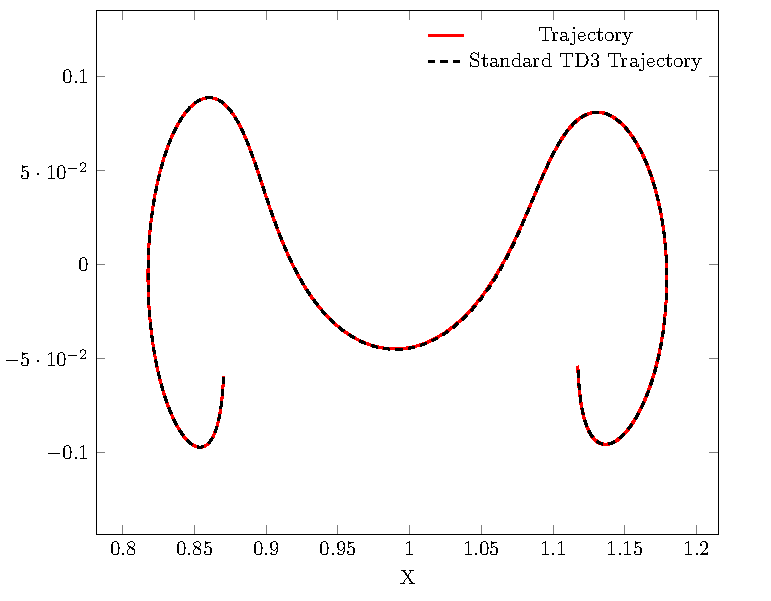
\includegraphics[width=.45\textwidth]{plots/td3/trajectory_force/plot_trajectory.pdf}}%
	\subfloat[\lr{MA-TD3} بازی مجموع‌صفر]{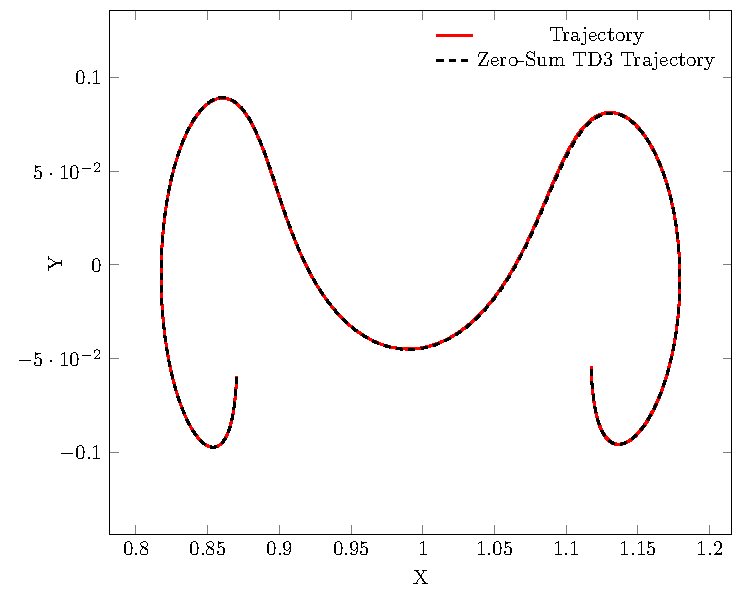
\includegraphics[width=.45\textwidth]{plots/td3/trajectory_force/plot_trajectory_zs.pdf}}%
	\caption{مسیر طی‌شده فضاپیما با \lr{TD3} استاندارد و نسخه بازی مجموع‌صفر \lr{MA-TD3}.}
\end{figure}

\subsection{مسیر و فرمان پیشران}
این بخش مسیر و پروفایل فرمان پیشران در طول زمان را برای هر دو نسخه \lr{TD3} ارائه می‌کند.
\begin{figure}[H]
	\centering
	\subfloat[\lr{TD3} استاندارد]{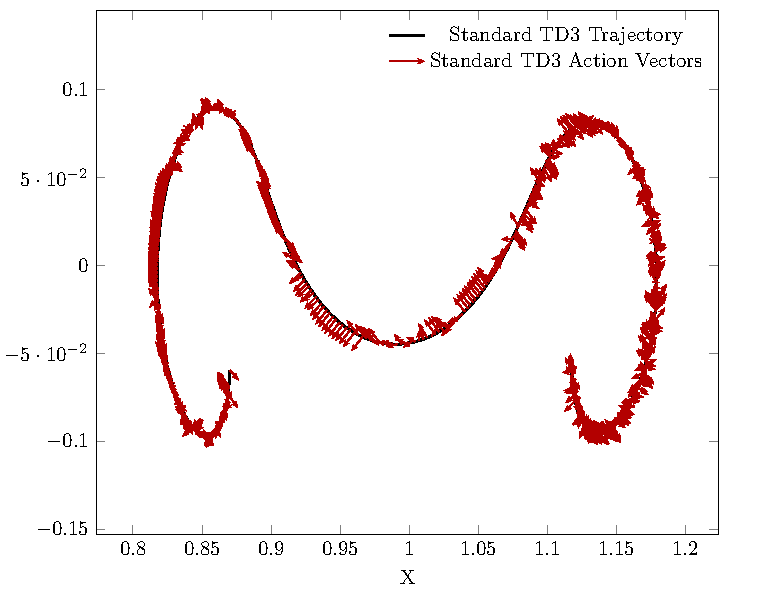
\includegraphics[width=.45\textwidth]{plots/td3/trajectory_force/plot_trajectory_force.pdf}}%
	\subfloat[\lr{MA-TD3} بازی مجموع‌صفر]{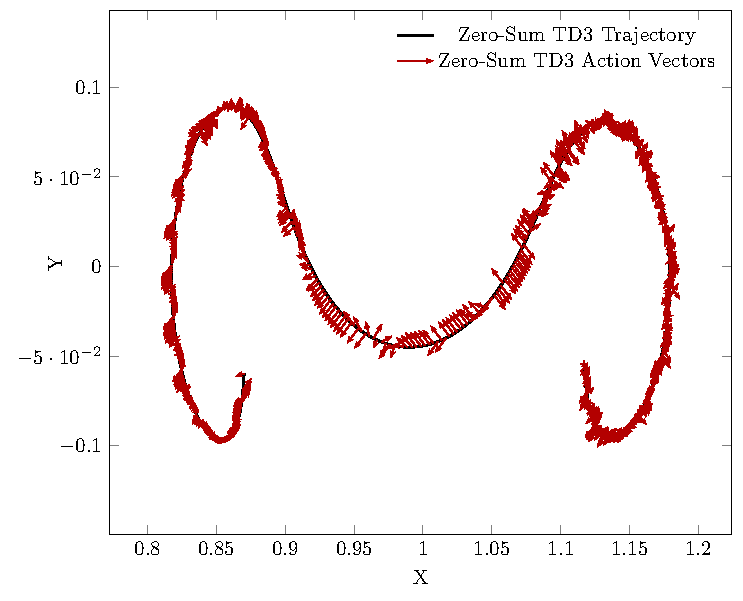
\includegraphics[width=.45\textwidth]{plots/td3/trajectory_force/plot_trajectory_force_zs.pdf}}%
	\caption{مسیر و فرمان پیشران فضاپیما در \lr{TD3} استاندارد و نسخه بازی مجموع‌صفر \lr{MA-TD3}.}
\end{figure}

\subsection{توزیع پاداش تجمعی}
این بخش نمودارهای ویولن توزیع پاداش تجمعی را در سناریوهای مختلف برای \lr{TD3} و \lr{MA-TD3} نمایش می‌دهد.
\begin{figure}[H]
	\centering
	% سطر اول
	\subfloat[شرایط اولیه تصادفی]{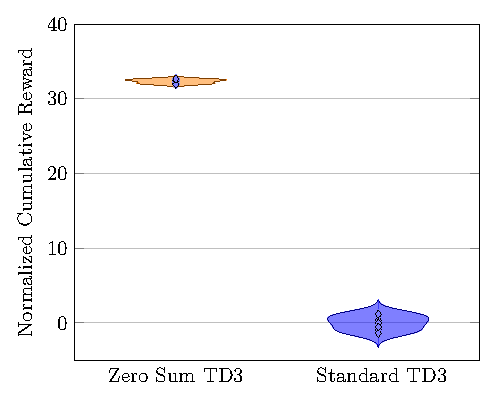
\includegraphics[width=.33\textwidth]{plots/td3/violin_plot/initial_condition_shift.pdf}}%
	\subfloat[اغتشاش در عملگرها]{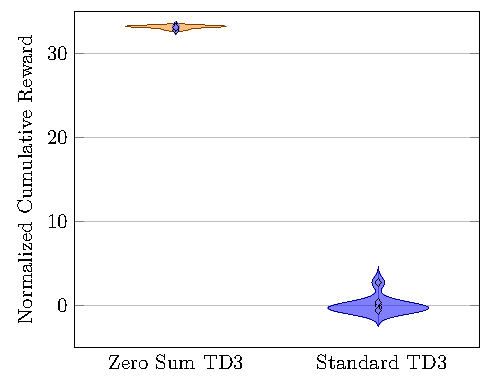
\includegraphics[width=.33\textwidth]{plots/td3/violin_plot/actuator_disturbance.pdf}}%
	\subfloat[عدم تطابق مدل]{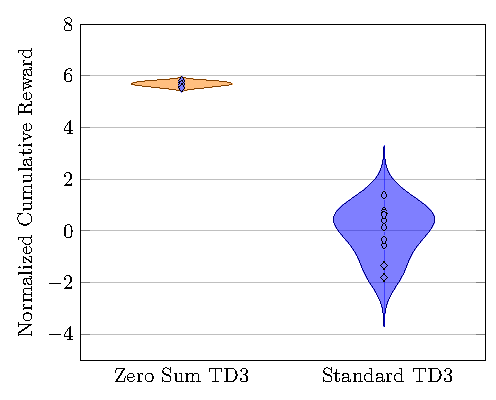
\includegraphics[width=.33\textwidth]{plots/td3/violin_plot/model_mismatch.pdf}}\\[1ex]
	% سطر دوم
	\subfloat[مشاهده ناقص]{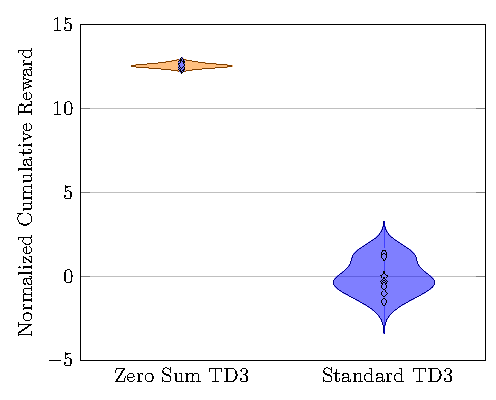
\includegraphics[width=.33\textwidth]{plots/td3/violin_plot/partial_observation.pdf}}%
	\subfloat[نویز حسگر]{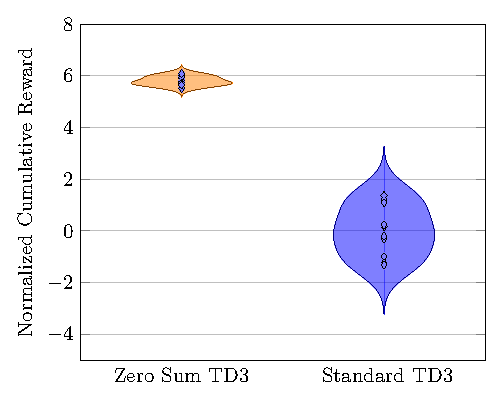
\includegraphics[width=.33\textwidth]{plots/td3/violin_plot/sensor_noise.pdf}}%
	\subfloat[تأخیر زمانی]{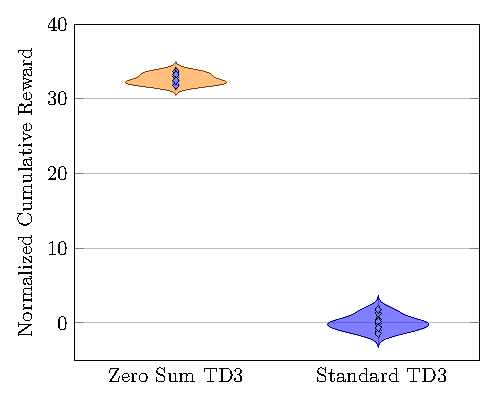
\includegraphics[width=.33\textwidth]{plots/td3/violin_plot/time_delay.pdf}}
	\caption{مقایسه توزیع پاداش تجمعی در سناریوهای مختلف برای \lr{TD3} و \lr{MA-TD3}.}
	\label{fig:td3_robustness_violin}
\end{figure}

\subsection{مقایسه عددی}
این بخش شاخص‌های عددی را گزارش می‌کند؛ نتایج بر اساس 100 اجرای مستقل شبیه‌سازی برای هر سناریو به‌دست آمده‌اند.
\begin{table}[H]
	\centering
	\setlength{\tabcolsep}{3pt}
	\small
	\begin{tabular}{@{} R{3.2cm} *{8}{C{1.05cm}} @{}}
		\toprule
		\multirow{2}{*}{\makecell[r]{سناریو}}
		& \multicolumn{2}{c}{پاداش تجمعی} & \multicolumn{2}{c}{مجموع خطای مسیر}
		& \multicolumn{2}{c}{مجموع تلاش کنترلی} & \multicolumn{2}{c}{احتمال شکست} \\
		\cmidrule(lr){2-3}\cmidrule(lr){4-5}\cmidrule(lr){6-7}\cmidrule(lr){8-9}
		& {\rotatebox[origin=c]{90}{\lr{TD3}}} & {\rotatebox[origin=c]{90}{\lr{MA-TD3}}}
		& {\rotatebox[origin=c]{90}{\lr{TD3}}} & {\rotatebox[origin=c]{90}{\lr{MA-TD3}}}
		& {\rotatebox[origin=c]{90}{\lr{TD3}}} & {\rotatebox[origin=c]{90}{\lr{MA-TD3}}}
		& {\rotatebox[origin=c]{90}{\lr{TD3}}} & {\rotatebox[origin=c]{90}{\lr{MA-TD3}}} \\
		\midrule
		شرایط اولیه تصادفی
		&
		$-2.95$ & ${-0.26}$ & $0.39$ & ${0.14}$ & $4.57$ & $4.57$ & $1.00$ & ${0.30}$\\
		اغتشاش در عملگرها
		&
		$0.56$ & ${0.73}$ & $0.02$ & ${0.00}$ & $2.66$ & $2.66$ & $0.00$ & $0.00$ \\
		عدم تطابق مدل
		&
		$-4.73$ & ${-3.30}$ & $0.47$ & $0.73$ & $5.41$ & $5.41$ & $1.00$ & $1.00$ \\
		مشاهده ناقص
		&
		$0.21$ & ${0.71}$ & $0.02$ & ${0.01}$ & $3.18$ & $3.18$ & $0.00$ & $0.00$ \\
		نویز حسگر
		&
		${-0.08}$ & $-2.93$ & ${0.11}$ & $3.19$ & $5.50$ & $5.50$ & ${0.00}$ & $1.00$ \\
		تأخیر زمانی
		&
		$0.55$ & ${0.67}$ & $0.01$ & $0.01$ & $4.57$ & $4.57$ & $0.00$ & $0.00$ \\
		\bottomrule
	\end{tabular}
	\caption{مقایسه عملکرد \lr{TD3} و \lr{MA-TD3} در سناریوهای مختلف مقاومت}
	\label{tab:td3_comparison}
\end{table}

الگوریتم \lr{TD3} در هر دو حالت عملکرد قابل توجهی دارد، اما نسخه بازی مجموع‌صفر آن بهبودهای معناداری در کیفیت مسیر و مصرف سوخت نشان می‌دهد. ثبات بیشتر این الگوریتم در مقایسه با \lr{DDPG} در هر دو نسخه قابل مشاهده است.